\documentclass{article}
\usepackage{/Library/Frameworks/R.framework/Resources/share/texmf/Sweave}
\title{Drawing Graphs for Incidence and Prevalence}
\author{Danny Kaplan}
\date{\today}
\begin{document}

\maketitle

Drawing graphs showing the progression of individuals through sickness
and death (or loss to follow-up), to help students estimate prevalence
and incidence.

Basic idea, for each person, generate a probability of sickness,
death, or loss.  Draw a line graph appropriately

Functions for getting sick, dying, or getting lost to follow up:
\begin{Schunk}
\begin{Sinput}
> sick = function(rate = 0.07) {
+     rexp(1, rate = rate)
+ }
> loss = function(rate = 0.02, lockout = 0.5) {
+     lockout + rexp(1, rate = rate)
+ }
> death = function(rate = 0.05) {
+     rexp(1, rate = rate)
+ }
\end{Sinput}
\end{Schunk}

Put these together for one person, graphing out the result:
\begin{Schunk}
\begin{Sinput}
> one.person = function(loc = 1) {
+     S = sick()
+     L = loss()
+     D = death()
+     if (S <= L & S <= D) {
+         lines(c(0, min(10, S)), c(loc, loc), col = "gray", lwd = 3)
+         L = loss()
+         D = death(rate = 0.3)
+         if (S < 10) 
+             lines(c(S, min(10, S + min(D, L))), c(loc, loc), 
+                 col = "red", lwd = 5)
+     }
+     else {
+         S = 0
+         lines(c(0, min(10, min(D, L))), c(loc, loc), col = "gray", 
+             lwd = 3)
+     }
+     if (L < D) {
+         text(S + L + 0.2, loc, "?", col = "red")
+     }
+     else {
+         text(S + D, loc, "X", col = "black")
+     }
+ }
\end{Sinput}
\end{Schunk}


Plot out a lot of them.
\begin{Schunk}
\begin{Sinput}
> show.population = function(n) {
+     plot(1:10, xlim = c(0, 10), ylim = c(0, n), type = "n", yaxt = "n", 
+         ylab = "People", xlab = "Years of Follow Up")
+     for (k in 1:n) one.person(k)
+ }
\end{Sinput}
\end{Schunk}

\section{For the Groups to Work On}

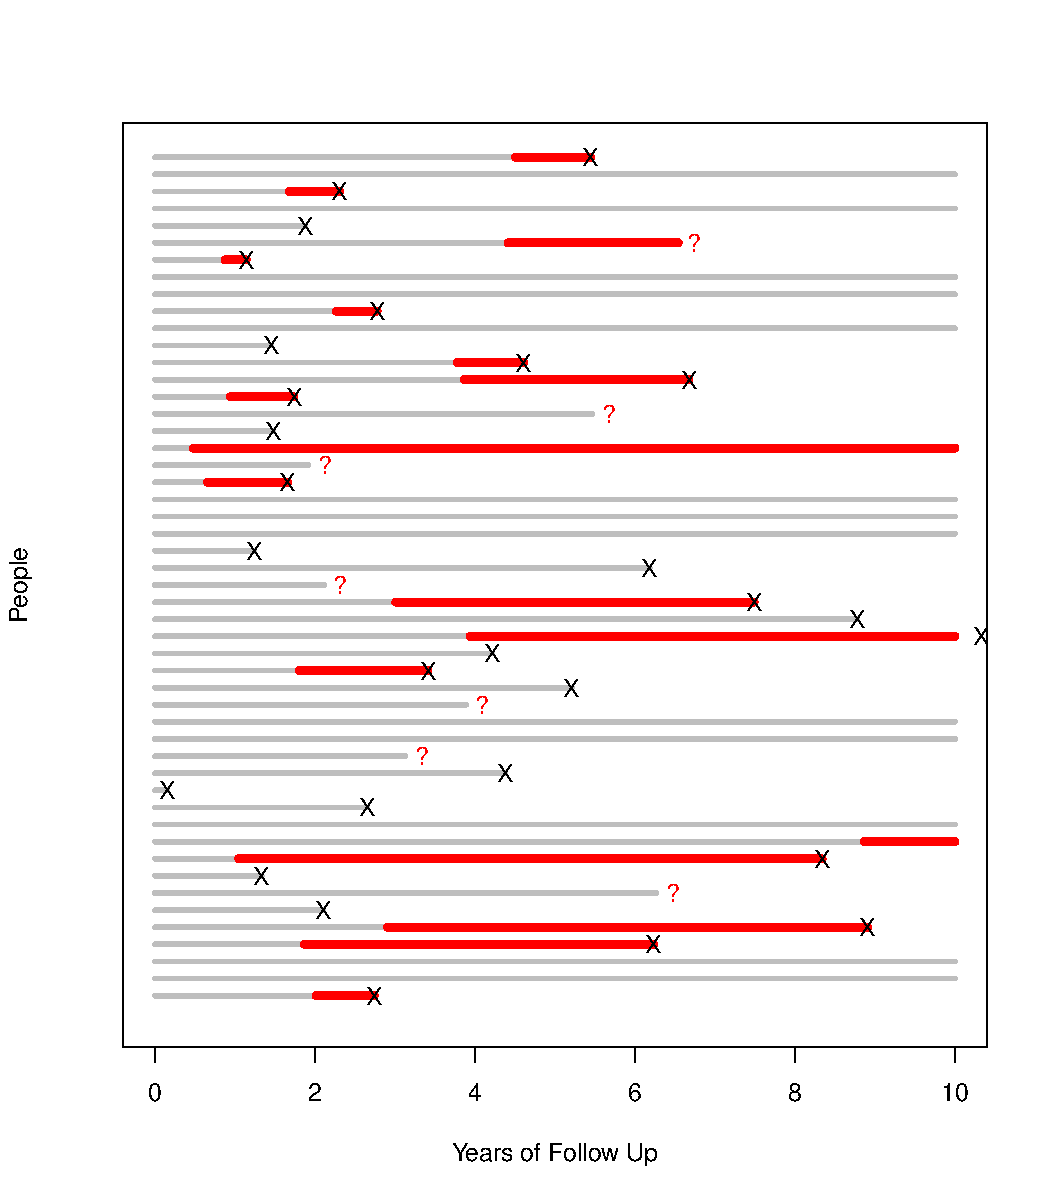
\includegraphics{incidence-graphs-one}

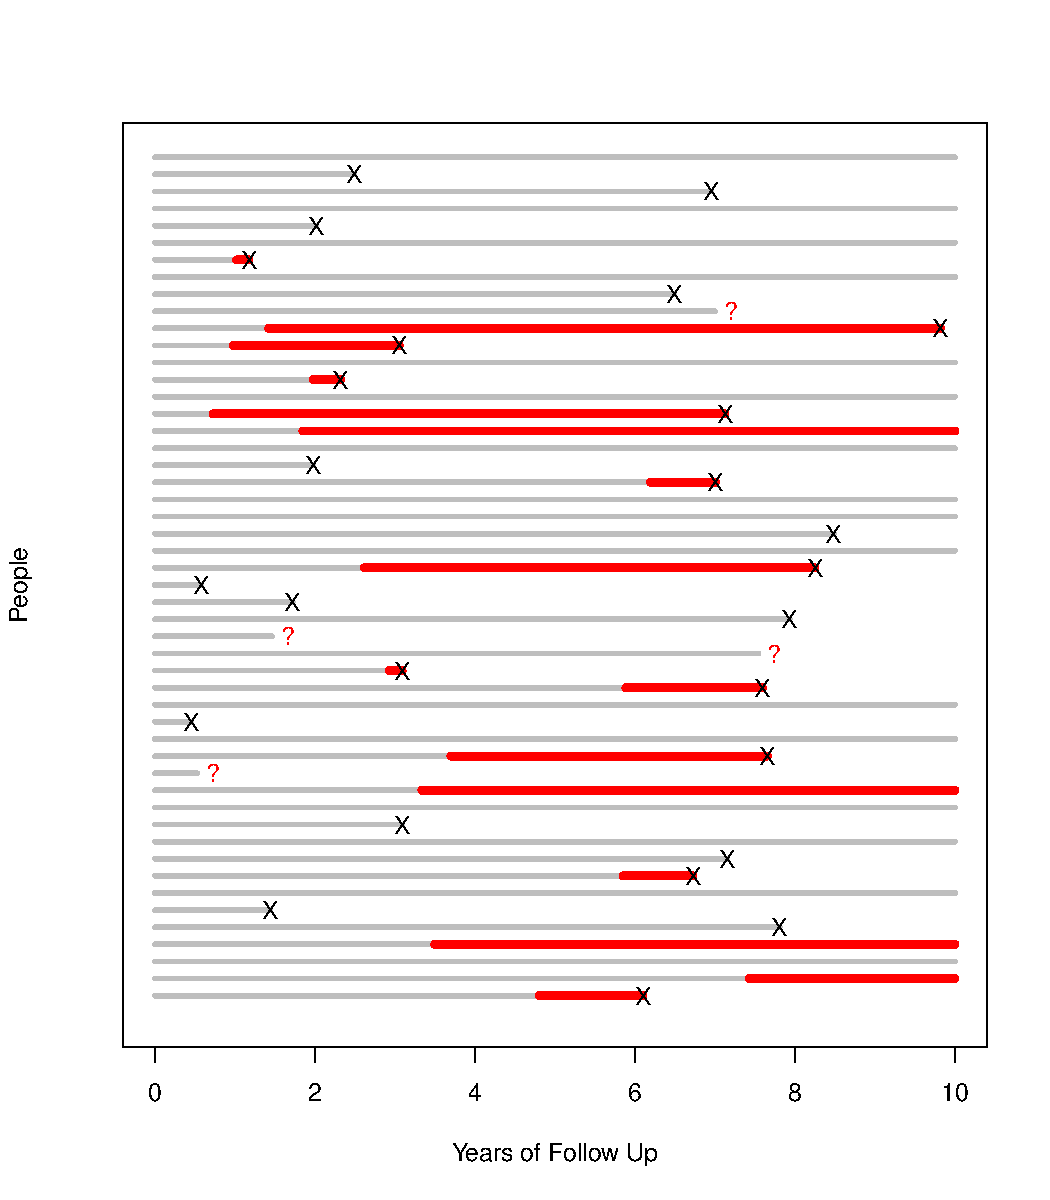
\includegraphics{incidence-graphs-two}

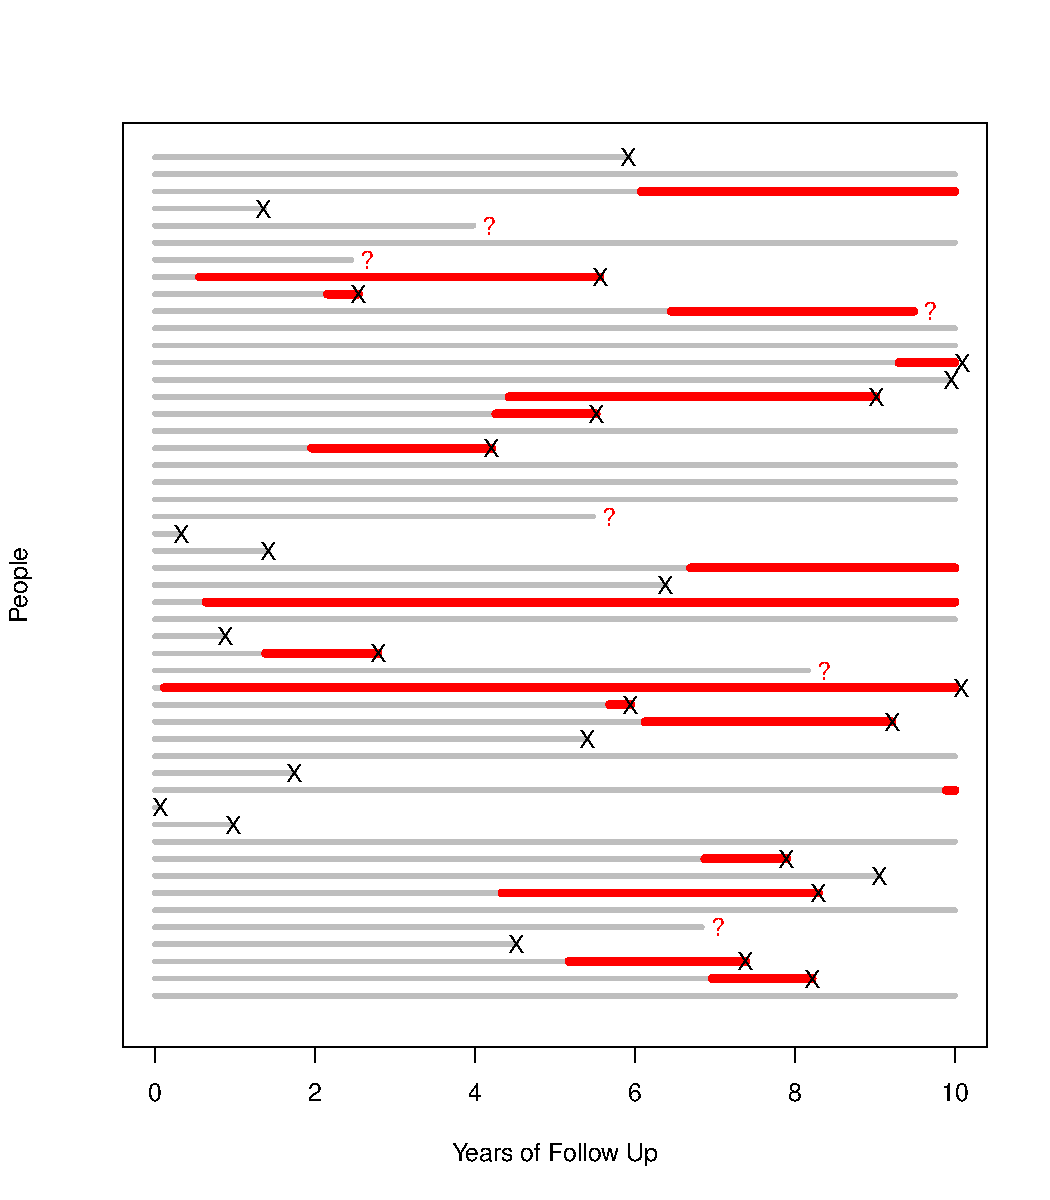
\includegraphics{incidence-graphs-three}

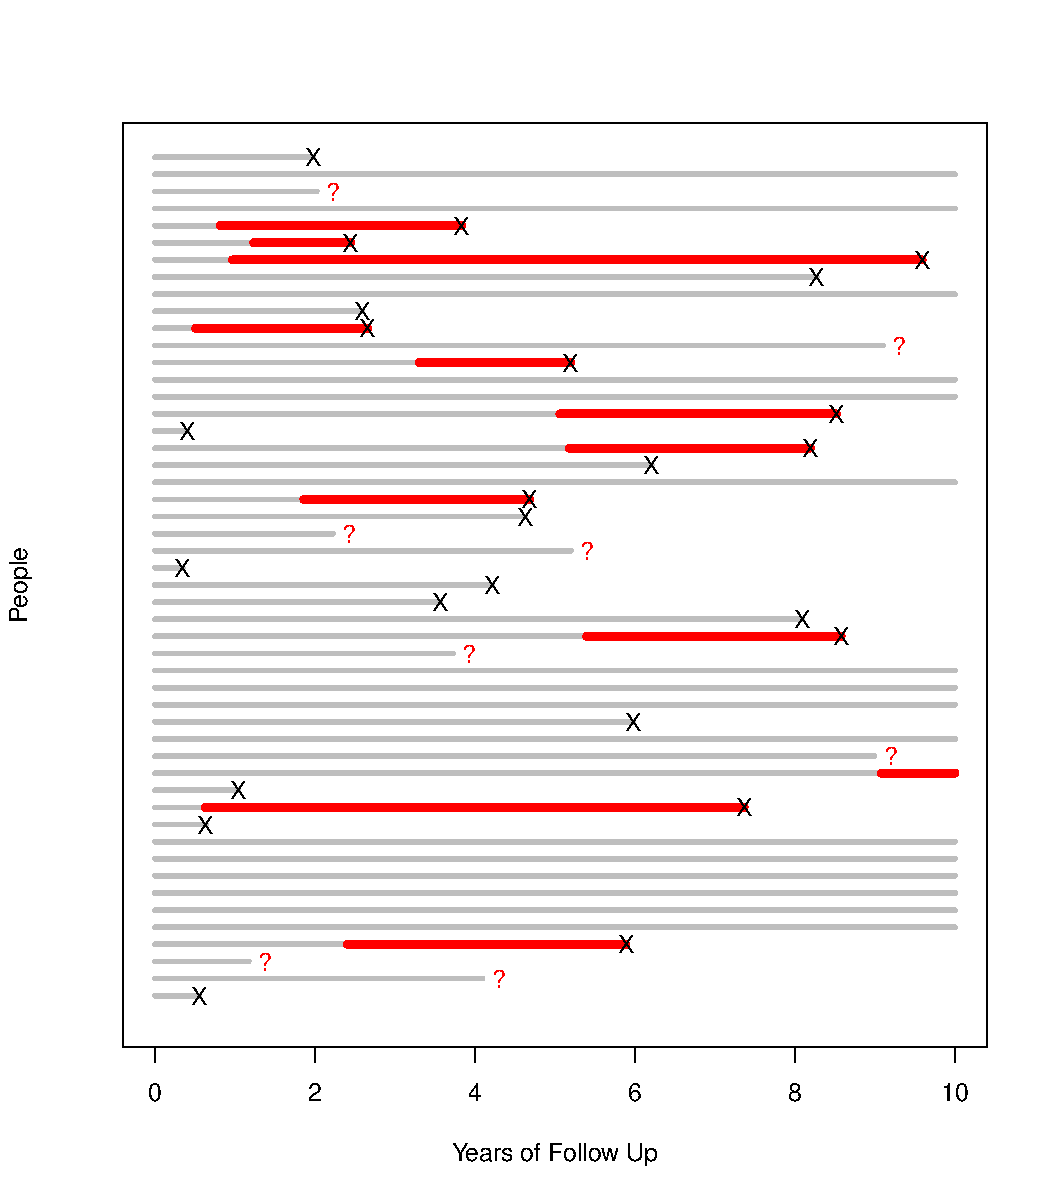
\includegraphics{incidence-graphs-four}

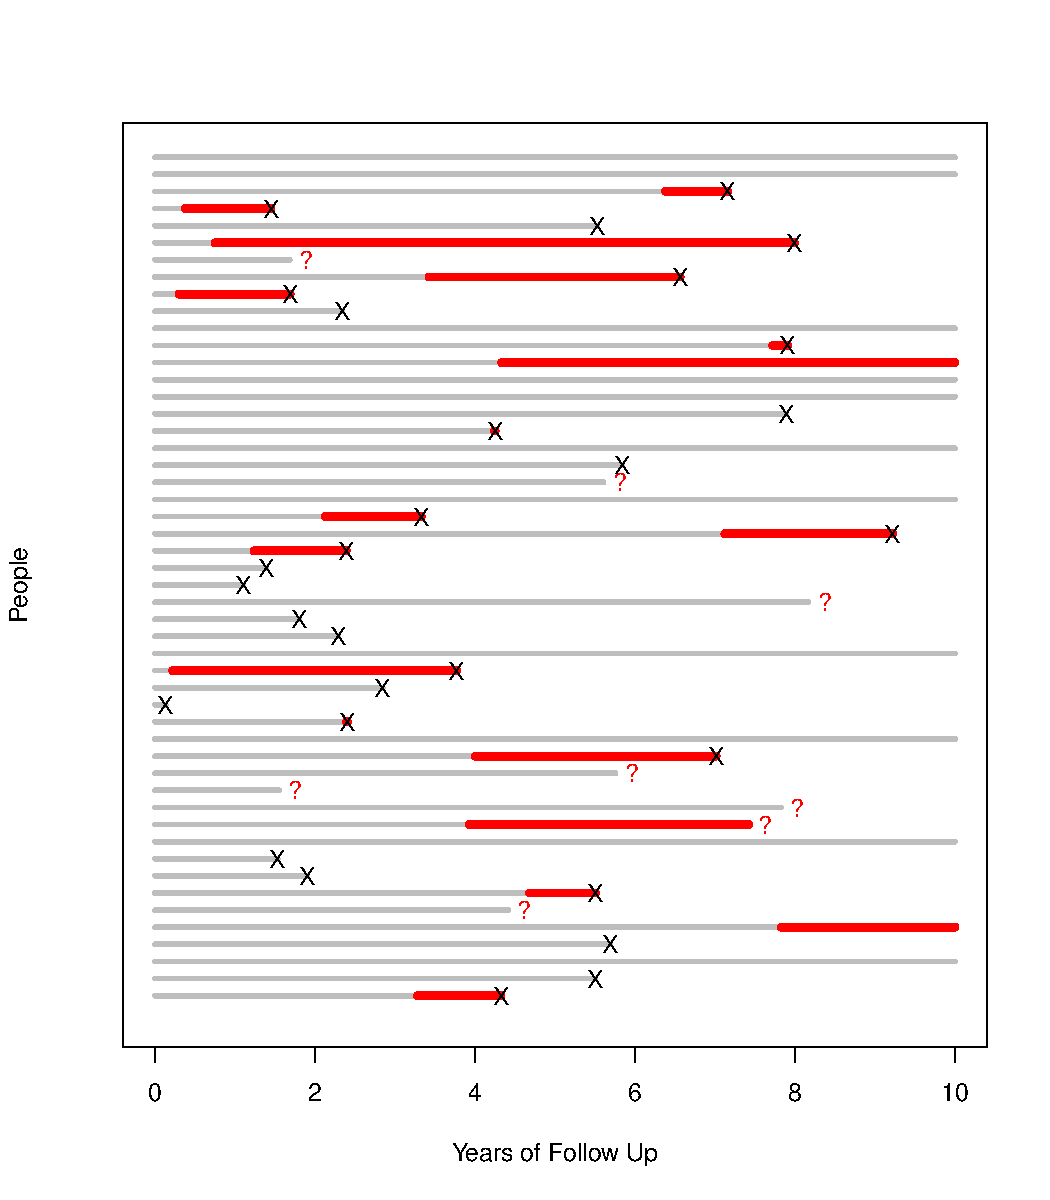
\includegraphics{incidence-graphs-five}

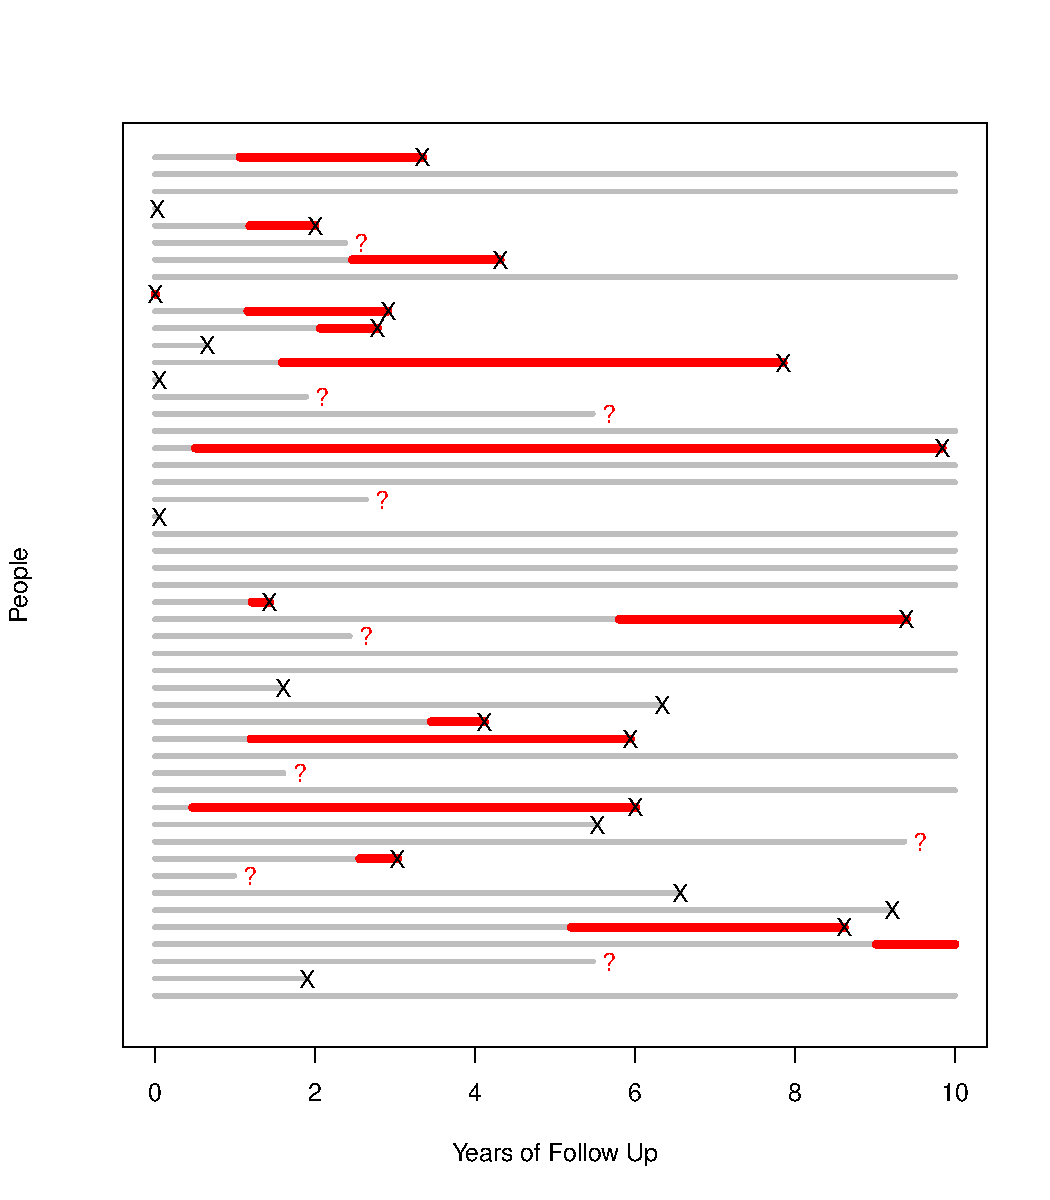
\includegraphics{incidence-graphs-six}

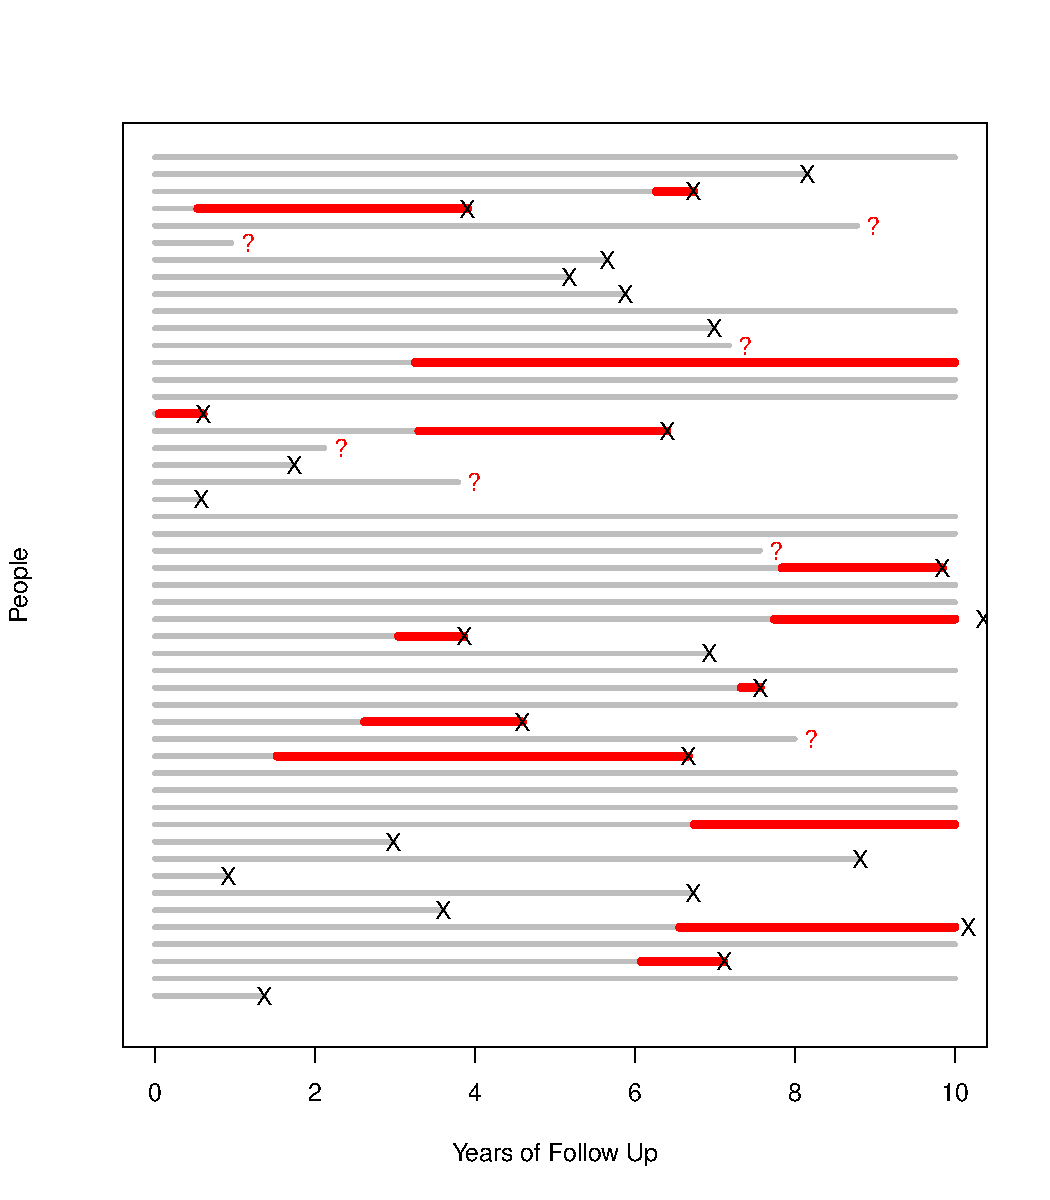
\includegraphics{incidence-graphs-seven}

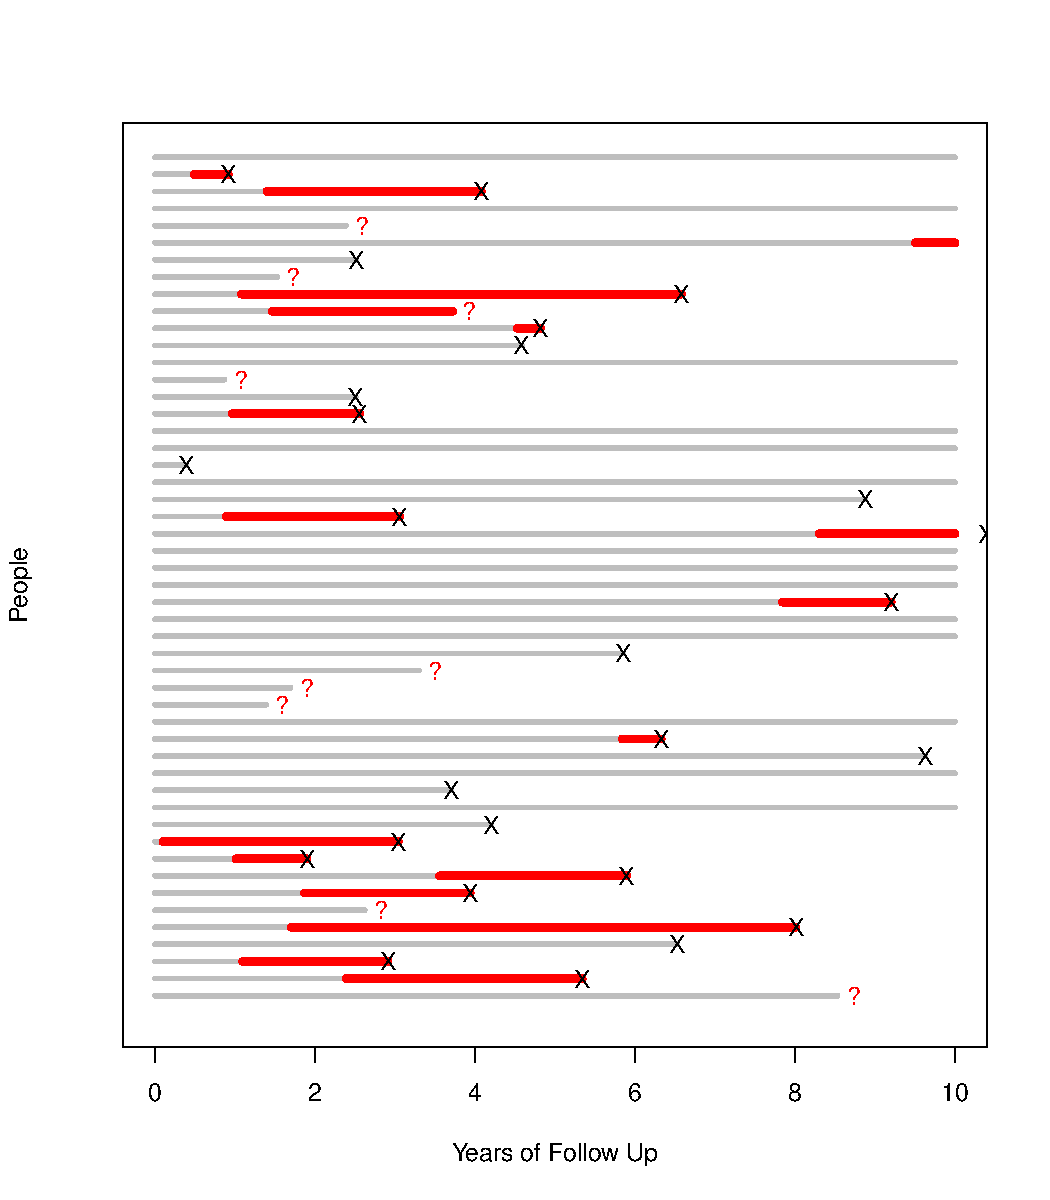
\includegraphics{incidence-graphs-eight}

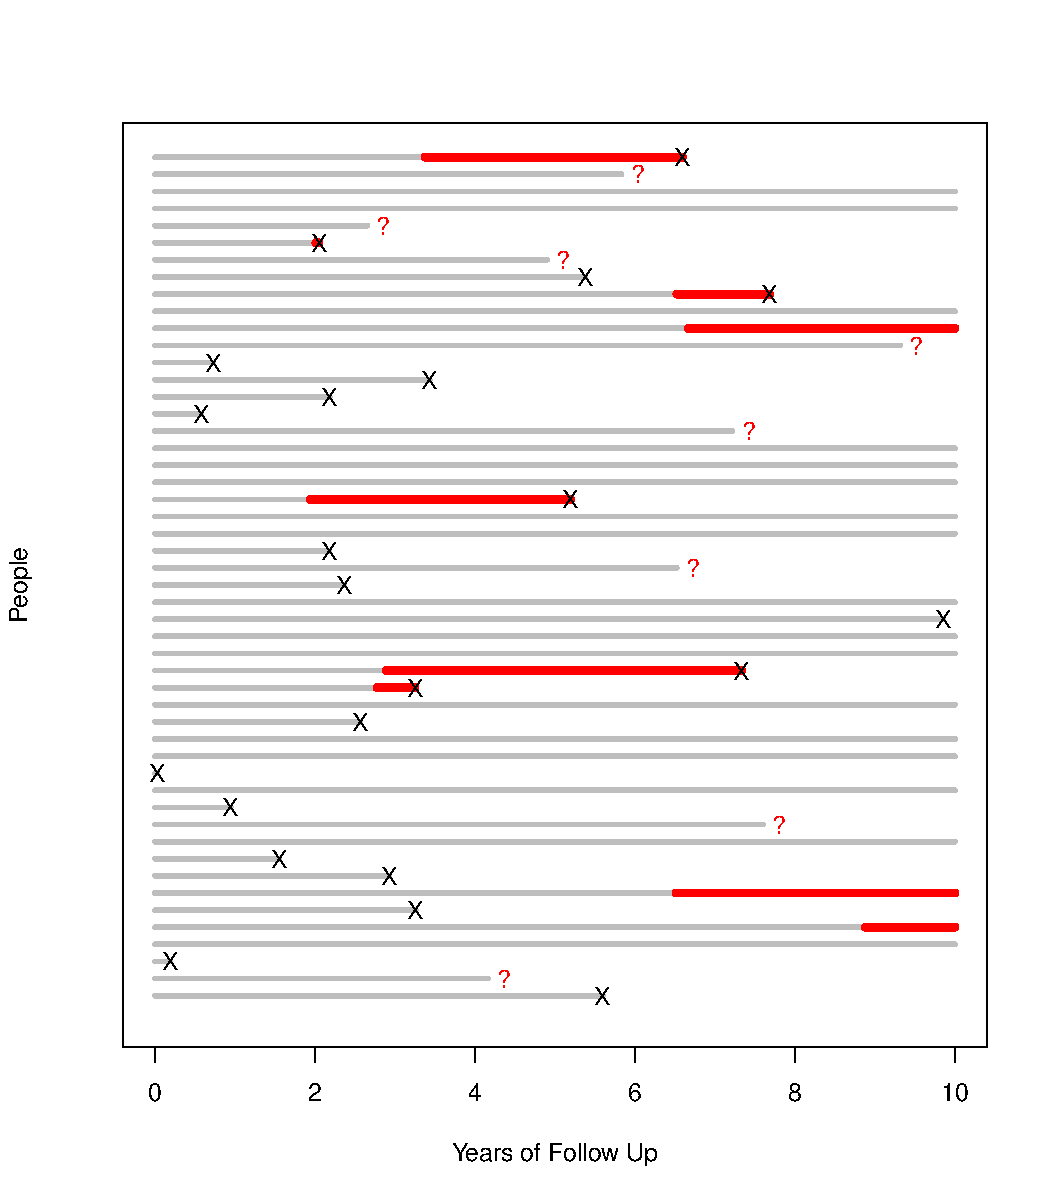
\includegraphics{incidence-graphs-nine}

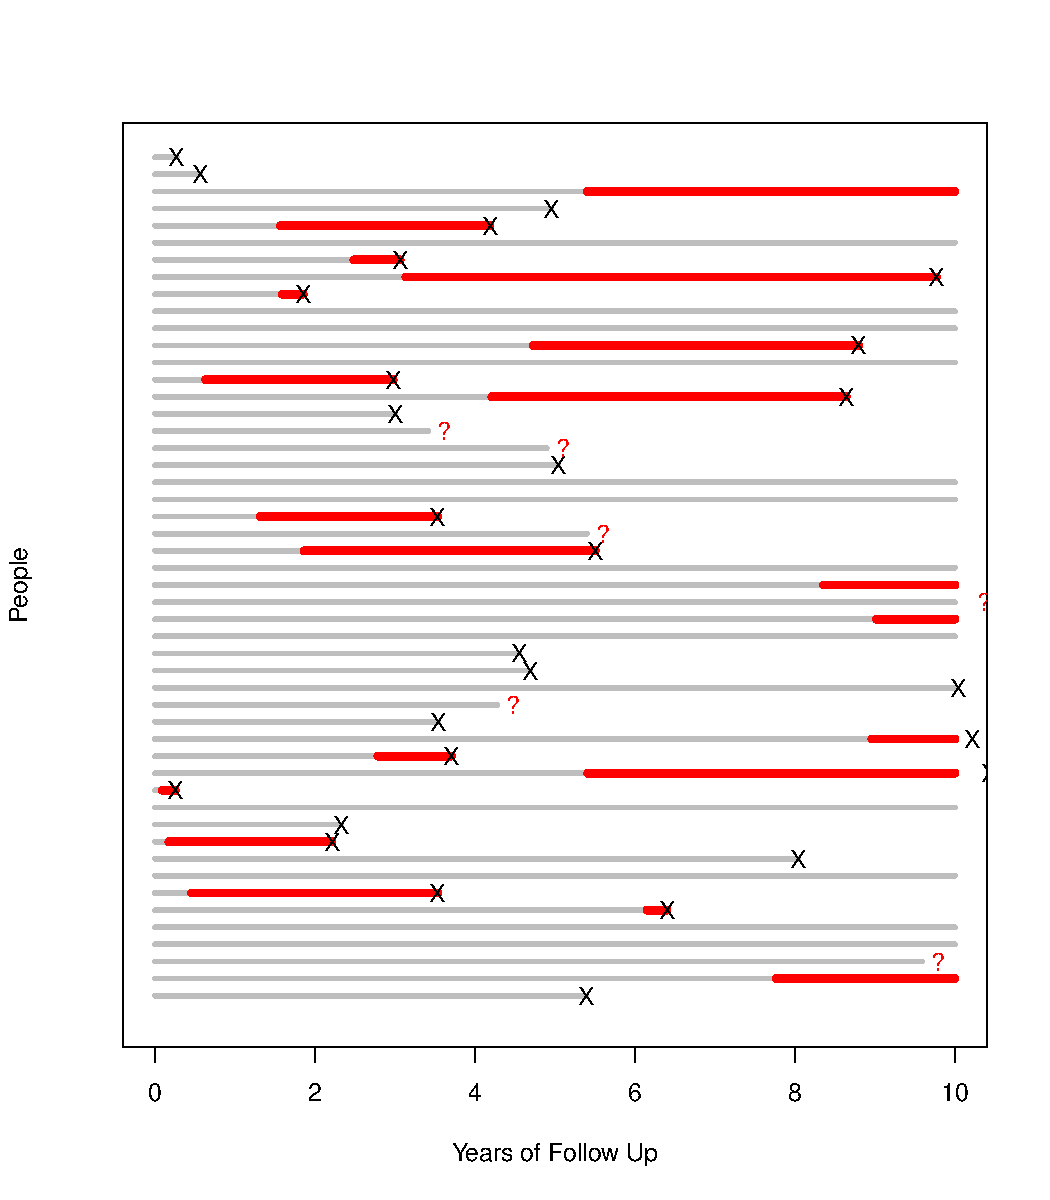
\includegraphics{incidence-graphs-ten}

\begin{Schunk}
\begin{Sinput}
> sick = function(rate = 0.03) {
+     rexp(1, rate = rate)
+ }
> loss = function(rate = 0.01, lockout = 0.5) {
+     lockout + rexp(1, rate = rate)
+ }
> death = function(rate = 0.025) {
+     rexp(1, rate = rate)
+ }
\end{Sinput}
\end{Schunk}

\section{For the In-Class Explanation}
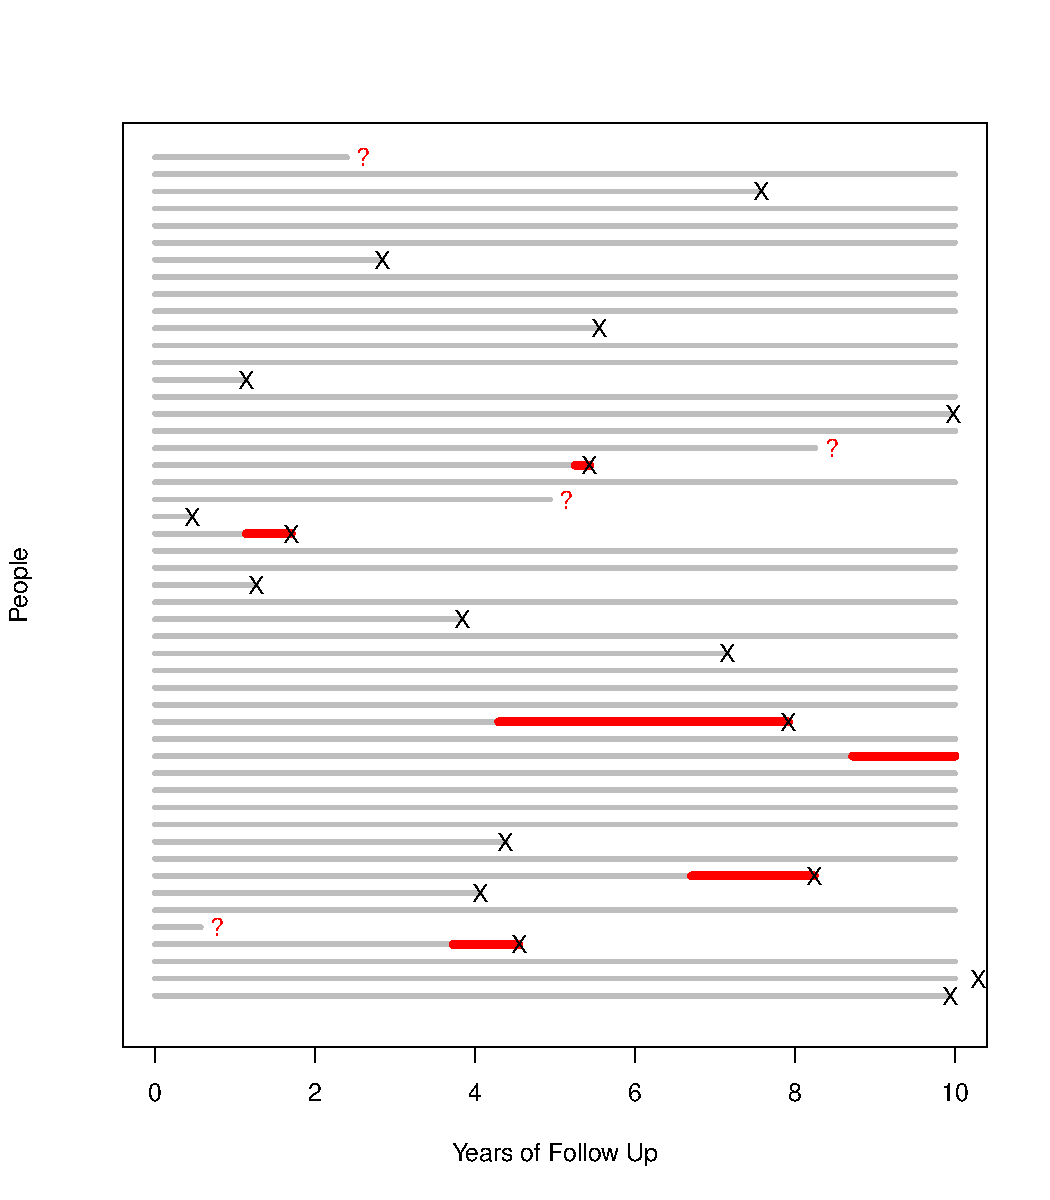
\includegraphics{incidence-graphs-inclass}


\end{document}
